\documentclass{beamer}
\usepackage{amsmath,amssymb}
\usepackage{tikz}
\usepackage{enumerate}
\usepackage{xcolor}
\usepackage{algorithm2e}

% Theorems
\usepackage{amsthm}
\renewcommand\qedsymbol{$\blacksquare$}
\makeatletter
\@ifclassloaded{article}{
    \newtheorem{definition}{Definition}[section]
    \newtheorem{example}{Example}[section]
    \newtheorem{theorem}{Theorem}[section]
    \newtheorem{corollary}{Corollary}[theorem]
    \newtheorem{lemma}{Lemma}[theorem]
}{
}
\makeatother

% Random Stuff
\setlength\unitlength{1mm}

\newcommand{\insertfig}[3]{
\begin{figure}[htbp]\begin{center}\begin{picture}(120,90)
\put(0,-5){\includegraphics[width=12cm,height=9cm,clip=]{#1.eps}}\end{picture}\end{center}
\caption{#2}\label{#3}\end{figure}}

\newcommand{\insertxfig}[4]{
\begin{figure}[htbp]
\begin{center}
\leavevmode \centerline{\resizebox{#4\textwidth}{!}{\input
#1.pstex_t}}
\caption{#2} \label{#3}
\end{center}
\end{figure}}

\long\def\comment#1{}

\newcommand\norm[1]{\left\lVert#1\right\rVert}
\DeclareMathOperator*{\argmin}{arg\,min}
\DeclareMathOperator*{\argmax}{arg\,max}

% bb font symbols
\newfont{\bbb}{msbm10 scaled 700}
\newcommand{\CCC}{\mbox{\bbb C}}

\newfont{\bbf}{msbm10 scaled 1100}
\newcommand{\CC}{\mbox{\bbf C}}
\newcommand{\PP}{\mbox{\bbf P}}
\newcommand{\RR}{\mbox{\bbf R}}
\newcommand{\QQ}{\mbox{\bbf Q}}
\newcommand{\ZZ}{\mbox{\bbf Z}}
\renewcommand{\SS}{\mbox{\bbf S}}
\newcommand{\FF}{\mbox{\bbf F}}
\newcommand{\GG}{\mbox{\bbf G}}
\newcommand{\EE}{\mbox{\bbf E}}
\newcommand{\NN}{\mbox{\bbf N}}
\newcommand{\KK}{\mbox{\bbf K}}
\newcommand{\KL}{\mbox{\bbf KL}}

% Vectors
\renewcommand{\aa}{{\bf a}}
\newcommand{\bb}{{\bf b}}
\newcommand{\cc}{{\bf c}}
\newcommand{\dd}{{\bf d}}
\newcommand{\ee}{{\bf e}}
\newcommand{\ff}{{\bf f}}
\renewcommand{\gg}{{\bf g}}
\newcommand{\hh}{{\bf h}}
\newcommand{\ii}{{\bf i}}
\newcommand{\jj}{{\bf j}}
\newcommand{\kk}{{\bf k}}
\renewcommand{\ll}{{\bf l}}
\newcommand{\mm}{{\bf m}}
\newcommand{\nn}{{\bf n}}
\newcommand{\oo}{{\bf o}}
\newcommand{\pp}{{\bf p}}
\newcommand{\qq}{{\bf q}}
\newcommand{\rr}{{\bf r}}
\renewcommand{\ss}{{\bf s}}
\renewcommand{\tt}{{\bf t}}
\newcommand{\uu}{{\bf u}}
\newcommand{\ww}{{\bf w}}
\newcommand{\vv}{{\bf v}}
\newcommand{\xx}{{\bf x}}
\newcommand{\yy}{{\bf y}}
\newcommand{\zz}{{\bf z}}
\newcommand{\0}{{\bf 0}}
\newcommand{\1}{{\bf 1}}

% Matrices
\newcommand{\Ab}{{\bf A}}
\newcommand{\Bb}{{\bf B}}
\newcommand{\Cb}{{\bf C}}
\newcommand{\Db}{{\bf D}}
\newcommand{\Eb}{{\bf E}}
\newcommand{\Fb}{{\bf F}}
\newcommand{\Gb}{{\bf G}}
\newcommand{\Hb}{{\bf H}}
\newcommand{\Ib}{{\bf I}}
\newcommand{\Jb}{{\bf J}}
\newcommand{\Kb}{{\bf K}}
\newcommand{\Lb}{{\bf L}}
\newcommand{\Mb}{{\bf M}}
\newcommand{\Nb}{{\bf N}}
\newcommand{\Ob}{{\bf O}}
\newcommand{\Pb}{{\bf P}}
\newcommand{\Qb}{{\bf Q}}
\newcommand{\Rb}{{\bf R}}
\newcommand{\Sb}{{\bf S}}
\newcommand{\Tb}{{\bf T}}
\newcommand{\Ub}{{\bf U}}
\newcommand{\Wb}{{\bf W}}
\newcommand{\Vb}{{\bf V}}
\newcommand{\Xb}{{\bf X}}
\newcommand{\Yb}{{\bf Y}}
\newcommand{\Zb}{{\bf Z}}

% Calligraphic
\newcommand{\Ac}{{\cal A}}
\newcommand{\Bc}{{\cal B}}
\newcommand{\Cc}{{\cal C}}
\newcommand{\Dc}{{\cal D}}
\newcommand{\Ec}{{\cal E}}
\newcommand{\Fc}{{\cal F}}
\newcommand{\Gc}{{\cal G}}
\newcommand{\Hc}{{\cal H}}
\newcommand{\Ic}{{\cal I}}
\newcommand{\Jc}{{\cal J}}
\newcommand{\Kc}{{\cal K}}
\newcommand{\Lc}{{\cal L}}
\newcommand{\Mc}{{\cal M}}
\newcommand{\Nc}{{\cal N}}
\newcommand{\Oc}{{\cal O}}
\newcommand{\Pc}{{\cal P}}
\newcommand{\Qc}{{\cal Q}}
\newcommand{\Rc}{{\cal R}}
\newcommand{\Sc}{{\cal S}}
\newcommand{\Tc}{{\cal T}}
\newcommand{\Uc}{{\cal U}}
\newcommand{\Wc}{{\cal W}}
\newcommand{\Vc}{{\cal V}}
\newcommand{\Xc}{{\cal X}}
\newcommand{\Yc}{{\cal Y}}
\newcommand{\Zc}{{\cal Z}}

% Bold greek letters
\newcommand{\alphab}{\hbox{\boldmath$\alpha$}}
\newcommand{\betab}{\hbox{\boldmath$\beta$}}
\newcommand{\gammab}{\hbox{\boldmath$\gamma$}}
\newcommand{\deltab}{\hbox{\boldmath$\delta$}}
\newcommand{\etab}{\hbox{\boldmath$\eta$}}
\newcommand{\lambdab}{\hbox{\boldmath$\lambda$}}
\newcommand{\epsilonb}{\hbox{\boldmath$\epsilon$}}
\newcommand{\nub}{\hbox{\boldmath$\nu$}}
\newcommand{\mub}{\hbox{\boldmath$\mu$}}
\newcommand{\zetab}{\hbox{\boldmath$\zeta$}}
\newcommand{\phib}{\hbox{\boldmath$\phi$}}
\newcommand{\psib}{\hbox{\boldmath$\psi$}}
\newcommand{\thetab}{\hbox{\boldmath$\theta$}}
\newcommand{\taub}{\hbox{\boldmath$\tau$}}
\newcommand{\omegab}{\hbox{\boldmath$\omega$}}
\newcommand{\xib}{\hbox{\boldmath$\xi$}}
\newcommand{\sigmab}{\hbox{\boldmath$\sigma$}}
\newcommand{\pib}{\hbox{\boldmath$\pi$}}
\newcommand{\rhob}{\hbox{\boldmath$\rho$}}

\newcommand{\Gammab}{\hbox{\boldmath$\Gamma$}}
\newcommand{\Lambdab}{\hbox{\boldmath$\Lambda$}}
\newcommand{\Deltab}{\hbox{\boldmath$\Delta$}}
\newcommand{\Sigmab}{\hbox{\boldmath$\Sigma$}}
\newcommand{\Phib}{\hbox{\boldmath$\Phi$}}
\newcommand{\Pib}{\hbox{\boldmath$\Pi$}}
\newcommand{\Psib}{\hbox{\boldmath$\Psi$}}
\newcommand{\Thetab}{\hbox{\boldmath$\Theta$}}
\newcommand{\Omegab}{\hbox{\boldmath$\Omega$}}
\newcommand{\Xib}{\hbox{\boldmath$\Xi$}}

% mixed symbols
\newcommand{\sinc}{{\hbox{sinc}}}
\newcommand{\diag}{{\hbox{diag}}}
\renewcommand{\det}{{\hbox{det}}}
\newcommand{\trace}{{\hbox{tr}}}
\newcommand{\tr}{\trace}
\newcommand{\sign}{{\hbox{sign}}}
\renewcommand{\arg}{{\hbox{arg}}}
\newcommand{\var}{{\hbox{var}}}
\newcommand{\cov}{{\hbox{cov}}}
\renewcommand{\Re}{{\rm Re}}
\renewcommand{\Im}{{\rm Im}}
\newcommand{\eqdef}{\stackrel{\Delta}{=}}
\newcommand{\defines}{{\,\,\stackrel{\scriptscriptstyle \bigtriangleup}{=}\,\,}}
\newcommand{\<}{\left\langle}
\renewcommand{\>}{\right\rangle}
\newcommand{\Psf}{{\sf P}}
\newcommand{\T}{\top}
\newcommand{\m}[1]{\begin{bmatrix} #1 \end{bmatrix}}

\beamertemplatenavigationsymbolsempty
\begin{document}

\begin{frame}
    \frametitle{Convex Combination / Line Segment}
    \begin{center}
        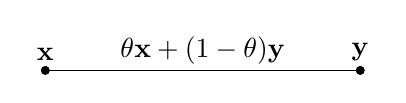
\begin{tikzpicture}
            \draw[fill=black] (0,0) circle (0.05) node[above] {$\xx$};
            \draw[fill=black] (4,0) circle (0.05) node[above] {$\yy$};
            \draw (0,0) -- (4,0);
            \draw (2,0.25) node {$\theta\xx + (1-\theta)\yy$};
        \end{tikzpicture}
    \end{center}
\end{frame}

\begin{frame}
    \frametitle{Convex Sets}
    \begin{center}
        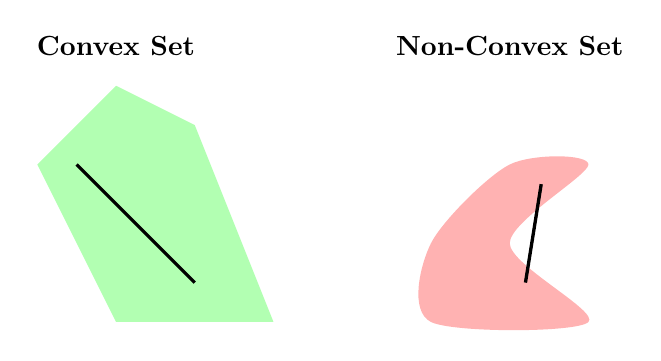
\begin{tikzpicture}
            \begin{scope}[shift={(-2,0)}]
                \draw (0,3.5) node {\textbf{Convex Set}};
                \fill[color=green!30] (0,0) -- (-1,2) -- (0,3) -- (1,2.5) -- (2,0)  -- cycle;
                \draw[very thick] (-0.5,2) -- (1,0.5);
            \end{scope}
            \begin{scope}[shift={(2,0)}]
                \draw (1,3.5) node {\textbf{Non-Convex Set}};
                \fill[color=red!30] plot [smooth cycle] coordinates {(0,1) (1,2) (2,2) (1,1) (2,0) (0,0)};
                \draw[very thick] (1.4,1.75) -- (1.2,0.5);
            \end{scope}
        \end{tikzpicture}
    \end{center}
\end{frame}

\begin{frame}
    \frametitle{Polytopes}

    Consider the set 
    \[
        S = \left\{\xx : \m{-1 & 0\\0 & -1\\1&2\\2&1}\xx \preceq \m{0\\0\\1\\1}\right\}
    \]
    \begin{center}
        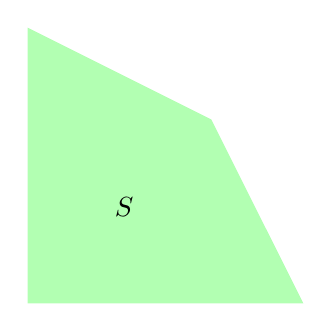
\begin{tikzpicture}[scale=3.5]
            \fill[color=green!30] (0,0) -- (1,0) -- (0.6666,0.6666) -- (0,1) -- cycle;
            \draw (0.35,0.35) node {$S$};
        \end{tikzpicture}
    \end{center}
\end{frame}

\begin{frame}
    \frametitle{Convex Functions}
    \begin{center}
        \begin{tikzpicture}
            \begin{scope}[shift={(-3.75,0)},scale=0.75]
                \draw[domain=-1.75:1.75,
                      smooth,
                      variable=\x,
                      blue] plot ({\x},{\x*\x/4});
                \draw (0, 4) node {\textbf{Convex Function}};
            \end{scope}
            \begin{scope}[shift={(0,0)},scale=0.75]
                \draw[domain=-1.75:1.75,
                      smooth,
                      variable=\x,
                      blue] plot ({\x},{-\x*\x/4 + 1});
                \draw (0, 4) node {\textbf{Concave Function}};
            \end{scope}
            \begin{scope}[shift={(3.75,0)},scale=0.75]
                \draw[domain=-1.75:1.75,
                      smooth,
                      variable=\x,
                      blue] plot ({\x},{\x*\x*\x/4 + 0.5});
                \draw (0, 4) node {\textbf{Neither}};
            \end{scope}
        \end{tikzpicture}
    \end{center}
\end{frame}

\begin{frame}
    \frametitle{Convex Function}
    \begin{center}
        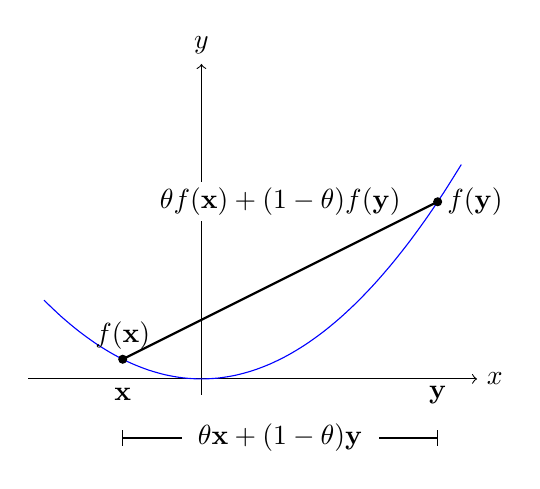
\begin{tikzpicture}
            \begin{scope}[shift={(-3,0)}]
                \draw[->] (-2.2,0) -- (3.5,0) node[right] {$x$};
                \draw[->] (0,-0.2) -- (0,4) node[above] {$y$};
                \draw[domain=-2:3.3,
                      smooth,
                      variable=\x,
                      blue] plot ({\x},{\x*\x/4});
                \fill[color=white] (-1,2) rectangle (2.75,2.5);
                \draw[fill=black] (-1,0.25) circle (0.05) node[above]{$f(\xx)$};
                \draw[fill=black] (3,2.25) circle (0.05) node[right]{$f(\yy)$};
                \draw (-1,-0.2) node {$\xx$};
                \draw (3,-0.2) node {$\yy$};
                \draw[thick] (-1,0.25) -- (3,2.25);
                \draw (1,2.25) node {$\theta f(\xx) + (1-\theta)f(\yy)$};
                \draw (1,-0.75) node {$\theta \xx + (1-\theta)\yy$};
                \draw (-1,-0.75) -- ++(0,0.1) -- ++(0,-0.2) -- ++(0,0.1) -- ++(0.75,0);
                \draw (3,-0.75) -- ++(0,0.1) -- ++(0,-0.2) -- ++(0,0.1) -- ++(-0.75,0);
            \end{scope}

            \begin{scope}[shift={(-3,0)}]
            \end{scope}
        \end{tikzpicture}
    \end{center}
\end{frame}

\begin{frame}
    \frametitle{Example Problem - Analytic Centering}
    Want to find some sort of `center' of a convex polygon (polytope) $A\xx \preceq \bb$:
    \begin{align*}
        \text{minimize: } f_0(\xx) = -\sum_{i}\log(\bb_i - a_i^\T\xx)
    \end{align*}

    \begin{figure}
        \centering
        \includegraphics[width=0.7\linewidth]{../fig/analytic_centering.pdf}
    \end{figure}
\end{frame}

\begin{frame}
    \frametitle{Example Problem - Least Squares Linear Regression}
    \begin{center}
        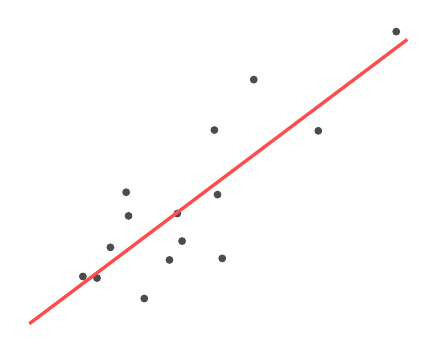
\begin{tikzpicture}
            % draw data
	    \fill[color=black!70] (-0.77,0.39) circle (0.05);
	    \fill[color=black!70] (-0.12,0.12) circle (0.05);
	    \fill[color=black!70] (0.35,1.18) circle (0.05);
	    \fill[color=black!70] (-1.14,-0.70) circle (0.05);
	    \fill[color=black!70] (-0.54,-0.96) circle (0.05);
	    \fill[color=black!70] (-1.32,-0.68) circle (0.05);
	    \fill[color=black!70] (0.85,1.82) circle (0.05);
	    \fill[color=black!70] (-0.74,0.09) circle (0.05);
	    \fill[color=black!70] (-0.97,-0.31) circle (0.05);
	    \fill[color=black!70] (-0.22,-0.47) circle (0.05);
	    \fill[color=black!70] (1.67,1.17) circle (0.05);
	    \fill[color=black!70] (0.45,-0.45) circle (0.05);
	    \fill[color=black!70] (0.39,0.36) circle (0.05);
	    \fill[color=black!70] (2.66,2.43) circle (0.05);
	    \fill[color=black!70] (-0.06,-0.23) circle (0.05);

            % draw line
            \draw[color=red!70, very thick] (-2,-1.28) -- (2.8,2.33);
        \end{tikzpicture}
    \end{center}
\end{frame}

\begin{frame}
    \frametitle{Example Problem - Logistic Regression}
    \begin{center}
        \begin{tikzpicture}
            \fill[color=black!70] (-1.01,-0.65) circle (0.05);
            \fill[color=black!70] (-3.20,-1.06) circle (0.05);
            \fill[color=black!70] (-2.00,-1.33) circle (0.05);
            \fill[color=black!70] (-1.91,-1.87) circle (0.05);
            \fill[color=black!70] (-2.33,-0.77) circle (0.05);
            \fill[color=black!70] (-1.82,-0.23) circle (0.05);
            \fill[color=black!70] (-2.06,-1.83) circle (0.05);
            \fill[color=black!70] (-1.61,-1.11) circle (0.05);
            \fill[color=black!70] (-1.93,-1.55) circle (0.05);
            \fill[color=black!70] (-2.23,-1.10) circle (0.05);
            \fill[color=black!70] (-1.16,-0.37) circle (0.05);
            \fill[color=black!70] (-2.09,-0.70) circle (0.05);
            \fill[color=black!70] (-2.82,-2.03) circle (0.05);
            \fill[color=black!70] (-2.28,-0.93) circle (0.05);
            \fill[color=black!70] (-2.05,-0.13) circle (0.05);

            \fill[color=orange!70] (-0.06,1.92) circle (0.05);
            \fill[color=orange!70] (1.30,0.58) circle (0.05);
            \fill[color=orange!70] (2.24,0.57) circle (0.05);
            \fill[color=orange!70] (3.37,0.60) circle (0.05);
            \fill[color=orange!70] (2.59,0.87) circle (0.05);
            \fill[color=orange!70] (2.19,0.33) circle (0.05);
            \fill[color=orange!70] (1.84,0.90) circle (0.05);
            \fill[color=orange!70] (1.80,0.57) circle (0.05);
            \fill[color=orange!70] (2.82,0.25) circle (0.05);
            \fill[color=orange!70] (2.10,1.11) circle (0.05);
            \fill[color=orange!70] (2.32,1.99) circle (0.05);
            \fill[color=orange!70] (2.79,1.25) circle (0.05);
            \fill[color=orange!70] (2.22,0.48) circle (0.05);
            \fill[color=orange!70] (3.48,0.29) circle (0.05);
            \fill[color=orange!70] (0.55,1.09) circle (0.05);
            \fill[color=orange!70] (0.99,1.03) circle (0.05);
            \fill[color=orange!70] (1.98,0.75) circle (0.05);
            \fill[color=orange!70] (-0.13,0.05) circle (0.05);
            \fill[color=orange!70] (2.29,1.12) circle (0.05);
            \fill[color=orange!70] (1.50,1.38) circle (0.05);
            \fill[color=orange!70] (0.85,1.04) circle (0.05);
            \fill[color=orange!70] (1.06,-0.26) circle (0.05);
            \fill[color=orange!70] (2.09,0.88) circle (0.05);
            \fill[color=orange!70] (2.19,1.12) circle (0.05);
            \fill[color=orange!70] (2.09,0.39) circle (0.05);

            % draw decision boundary
            \draw[color=red!70, very thick] (-1,2-0.5) -- (1,-2-0.5);
        \end{tikzpicture}
    \end{center}
\end{frame}

\begin{frame}
    \frametitle{Gradient Descent}
    \begin{center}
        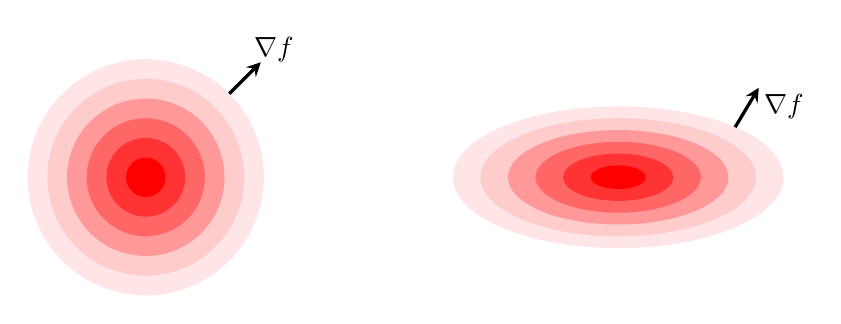
\begin{tikzpicture}
            \begin{scope}[shift={(-3,0)}]
                \fill[color=red!10] (0,0) circle (0.25*6);
                \fill[color=red!20] (0,0) circle (0.25*5);
                \fill[color=red!40] (0,0) circle (0.25*4);
                \fill[color=red!60] (0,0) circle (0.25*3);
                \fill[color=red!80] (0,0) circle (0.25*2);
                \fill[color=red!100] (0,0) circle (0.25*1);
                \draw[-stealth,very thick] ({1.5/sqrt(2)},{1.5/sqrt(2)}) -- ++(0.4,0.4);
                \draw ({2.3/sqrt(2)},{2.3/sqrt(2)}) node {$\nabla f$};
            \end{scope}

            \begin{scope}[shift={(3,0)}]
                \fill[color=red!10] (0,0) ellipse (0.35*6 and 0.15*6);
                \fill[color=red!20] (0,0) ellipse (0.35*5 and 0.15*5);
                \fill[color=red!40] (0,0) ellipse (0.35*4 and 0.15*4);
                \fill[color=red!60] (0,0) ellipse (0.35*3 and 0.15*3);
                \fill[color=red!80] (0,0) ellipse (0.35*2 and 0.15*2);
                \fill[color=red!100] (0,0) ellipse (0.35*1 and 0.15*1);
                \draw[-stealth,very thick] ({0.35*6/sqrt(2)},{0.15*6/sqrt(2)}) -- ++(0.15*2,0.25*2);
                \draw ({0.35*8.5/sqrt(2)},{0.15*8.5/sqrt(2)}) node {$\nabla f$};
            \end{scope}
        \end{tikzpicture}
    \end{center}
\end{frame}

\begin{frame}
    \frametitle{Gradient Descent}
    \begin{algorithm}[H]
        \SetKwInOut{Input}{input}\SetKwInOut{Output}{output}
        \textbf{Gradient Descent}\\
        \Input{$f$, $\nabla f$, $\eta(t)$, starting point $\xx_0$, tolerance $\epsilon$}
        \Output{optimal point $\xx^\star$}
        $t \leftarrow 0$\\
        \While{$|| \nabla f ||_2 \geq \epsilon$}{
            $\xx_{t+1} \leftarrow \xx_t - \eta(t)\nabla f(\xx_t)$\\
            $t \leftarrow t + 1$
        }
        \textbf{return } $\xx^\star = \xx_{t+1}$
    \end{algorithm}
\end{frame}

\begin{frame}
    \frametitle{Newton's Method}

    \begin{center}
        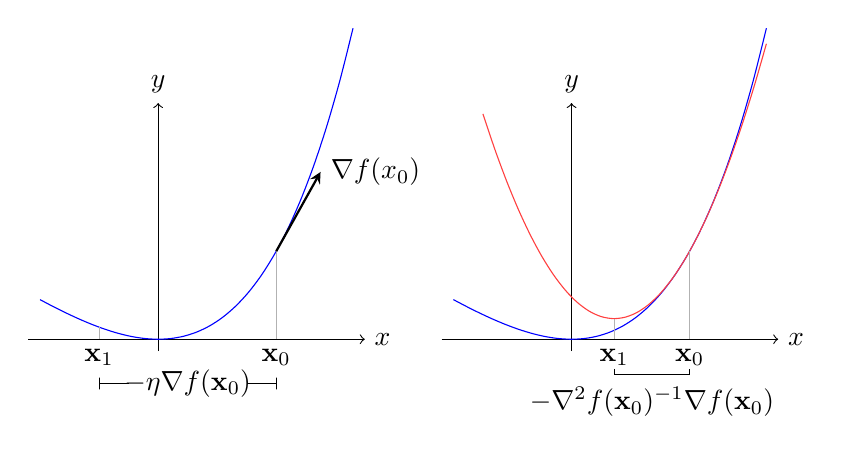
\begin{tikzpicture}[scale=0.75]
            \begin{scope}[shift={(-3.5,0)}]
                \draw[->] (-2.2,0) -- (3.5,0) node[right] {$x$};
                \draw[->] (0,-0.2) -- (0,4) node[above] {$y$};
                \draw[domain=-2:3.3,
                      smooth,
                      variable=\x,
                      blue] plot ({\x},{exp(\x/5)*\x*\x/4});
                \draw (2,0) node[below]{$\xx_0$};
                \draw[color=black!30] (2,0) -- (2,{exp(2/5)});
                \draw[thick,-stealth] (2,1.49) -- ++(0.75,{1.79*0.75}) node[right] {$\nabla f(x_0)$};
                \draw (-1,0) node[below]{$\xx_1$};
                \draw[color=black!30] (-1,0) -- (-1,{exp(-1/5)/4});
                \draw (-1,-0.75) -- ++(0,0.1) -- ++(0,-0.2) -- ++(0,0.1) -- ++(0.5,0);
                \draw (2,-0.75) -- ++(0,0.1) -- ++(0,-0.2) -- ++(0,0.1) -- ++(-0.5,0);
                \draw (0.5,-0.75) node {$-\eta\nabla f(\xx_0)$};
            \end{scope}
            \begin{scope}[shift={(3.5,0)}]
                \draw[->] (-2.2,0) -- (3.5,0) node[right] {$x$};
                \draw[->] (0,-0.2) -- (0,4) node[above] {$y$};
                \draw[domain=-2:3.3,
                      smooth,
                      variable=\x,
                      blue] plot ({\x},{exp(\x/5)*\x*\x/4});
                \draw[domain=-1.5:3.3,
                      smooth,
                      variable=\x,
                      red!75] plot ({\x},{1.49182 + 1.79019*(\x-2) + 0.701158*(\x-2)*(\x-2)});
                \draw (2,0) node[below] {$\xx_0$};
                \draw[color=black!30] (2,0) -- (2,1.49182);
                \draw (0.723404,0) node[below] {$\xx_1$};
                \draw[color=black!30] (0.723404,0) -- (0.723404,0.34915);
                \draw (0.723404,-0.5) -- ++(0,-0.1) -- ++({2-0.723404},0) -- ++(0,0.1);
                \draw ({(2+0.723404)/2},-0.65) node[below] {$-\nabla^2f(\xx_0)^{-1}\nabla f(\xx_0)$};
            \end{scope}
        \end{tikzpicture}
    \end{center}
\end{frame}

\begin{frame}
    \frametitle{Newton's Method}
    \begin{algorithm}[H]
        \SetKwInOut{Input}{input}\SetKwInOut{Output}{output}
        \textbf{Newton's Method}\\
        \Input{$f$, $\nabla f$, $\nabla^2f$, starting point $\xx_0$, tolerance $\epsilon$}
        \Output{optimal point $\xx^\star$}
        $t \leftarrow 0$\\
        \While{$|| \nabla f ||_2 \geq \epsilon$}{
            solve $\nabla^2 f(\xx_t) \dd_t = \nabla f(\xx_t)$ for $\dd_t$\\
            $\xx_{t+1} \leftarrow \xx_t - \dd_t$\\
            $t \leftarrow t + 1$
        }
        \textbf{return } $\xx^\star = \xx_{t+1}$
    \end{algorithm}
\end{frame}

\end{document}
